% !TEX root = deckblatt2b.tex

\section{RC-Tiefpass}

\begin{figure}[H]
  \begin{center}
    %\tikzset{component/.style={draw,thick,circle,fill=white,minimum size =0.75cm,inner sep=0pt}}
    \begin{circuitikz}
      \draw (0,2)
      to[R=$R$] (3,2)
      to[short] (6,2);
      \draw (4,2)
      to[C=$C$] (4,0);
      \draw (0,0)
      to[short] (6,0);
      \draw (0,1.8)
       to[short] (0,0.7) node[vee] {};
      \draw (-0.5,1) node[] {$U_e$};
      \draw (6,1.8)
       to[short] (6,0.7) node[vee] {};
      \draw (6.5,1) node[] {$U_a$};
    \end{circuitikz}
    \caption{RC-Tiefpass 1.Ordnung}
    \vspace{1cm}
    Das Schaltbild zeigt den Messaufbau des RC-Tiefpassfilters 1.Ordnung.\\
    $R=22k\Omega, C=1nF, U_e=1V$\\
  \end{center}
\end{figure}

\subsection{Sprungantwort}
\begin{figure}[H]
 \begin{center}
  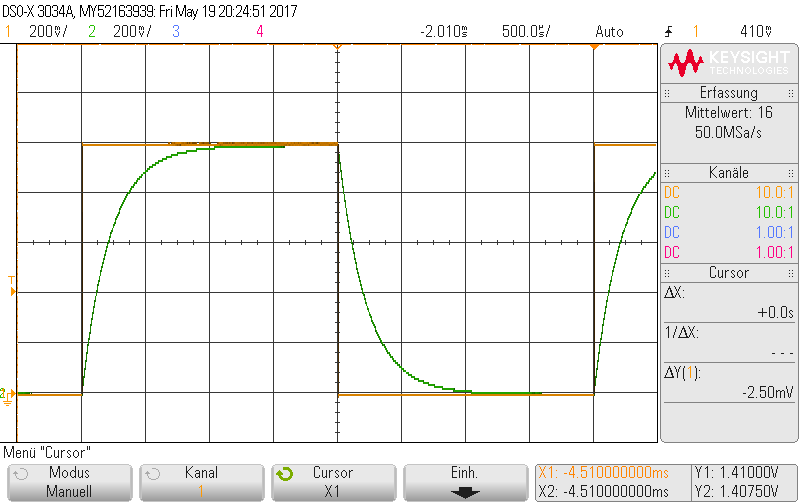
\includegraphics[height=6cm,width=12cm]{Oszi_Bilder/RC_Sprung}
 \end{center}
 \caption{Sprungantwort RC-Tiefpass}
\end{figure}
\noindent
In der Abbildung der Sprungantwort sind die exponentiellen Lade- und Entladekurven des Kondesators zu sehen. \\
\begin{align*}
 U_{charge} &= U_e(1 - e^{-\frac{t}{\tau}})\\
 U_{drain} &= U_e e^{-\frac{t}{\tau}}\\
 \tau &= RC
\end{align*}
\noindent
Die Zeitkonstante kann direkt aus der Sprungantwort abgelesen werden, indem man die Zeitdifferenz von $U_e=0$ bis $U_C \approx 0,6U_e$ misst. Daraus ergibt
sich ein $\tau_{gemessen}$ von $210\mu s$, dass gegenüber einem $\tau_{berechnet}$ von $220\mu s$ steht. Der Messfehler ergibt sich durch, ungenaues ablesen mit dem Cursor und Bauteiltoleranzen.\\

\subsection{Bode Diagramm}

Das Bode Diagramm zeigt den Verlauf der Dämpfung und des Phasenwinkels des Filters in abhängigkeit der Frequenz.\\
\begin{figure}[H]
  \centering
  \begin{tikzpicture}
    \begin{axis}[width=15cm, height=7cm, xmode=log, xmin=10, xmax=1e7, xlabel={$Hz$}, ylabel={dB},y tick label style={grid=major}]
      \addplot table[x=Frequenz, y=dB, col sep=comma] {csv_files/RC_dB.csv};
      \node[label={260:{$f_g$}},rectangle,fill=blue,inner sep=3pt] at (axis cs:723.43,-3) {};
    \end{axis}
  \end{tikzpicture}
  \caption{Bode Diagramm RC-Tiefpass, Dämpfung}
\end{figure}
\noindent
Die niedrigen Frequenzen werden vom Tiefpassfilter ungedämpft durchgelassen. Erst ab der Grenzfrequenz, von $f_g = \frac{1}{2\pi RC} = 723,43Hz$, nimmt die Dämpfung
mit $-20dB/DEK$ zu. Ab $100kHz$ war die Dämpfung mit dem Oszilloskop nahezu nicht mehr messbar. \\

\begin{figure}[H]
  \centering
  \begin{tikzpicture}
    \begin{axis}[width=15cm, height=7cm, xmode=log, xmin=10, xmax=1e7, xlabel={$Hz$}, ylabel={$\phi$},y tick label style={grid=major}]
      \addplot table[x=Frequenz, y=Phi, col sep=comma] {csv_files/RC_Phi.csv};
      \node[label={260:{$f_g$}},rectangle,fill=blue,inner sep=3pt] at (axis cs:723.43,-45) {};
    \end{axis}
  \end{tikzpicture}
  \caption{Bode Diagramm RC-Tiefpass, Phasengang}
\end{figure}
\noindent
Der Phasengang verläuft von $0^\circ$ bis $-90^\circ$. Auch hier wurde die Messung ab $100kHz$ sehr ungenau. Die Grenzfrequenz liegt hier bei $-45^\circ$.\\
\\
Die Messergebnisse des RC-Tiefpassfilters 1.Ordnung stimmen, bis auf kleine Abweichungen durch Messfehler und Bauteiltoleranzen, weitest gehend mit der Simmulation überein.
Nur bei hohen Frequenzen, ab ca $100kHz$, gab es bei der Messung der Ausgangsspannung und des Phasenwinkels Ungenauigkeiten, da durch die fortgeschrittene Dämpfung das
Ausgangssignal kaum mehr zu messen war. \\
